\section{Experiment Design and Results}
\label{sec:experiment}

\subsection{Implementation}

Our prototype uses: Circom~2.0 $+$ circomlib~2.0.5 (Poseidon, LessEqThan,
Switcher); snarkjs~0.7.6 for Groth16 on BN254; custom \texttt{ffjavascript}-based
true batch verification (Algorithm~\ref{alg:batch_verify}); and a local Powers of
Tau (pot14, 2-contribution ceremony) trusted setup.

\textbf{Hardware.} All benchmarks are conducted directly on a \textbf{Raspberry Pi~4
Model~B Rev~1.2} (ARM Cortex-A72 @ 1.8\,GHz, 4-core, 3.76\,GB RAM, aarch64,
Debian GNU/Linux 13), serving as our OBU-class target platform.
For the rapidsnark evaluation, the native C++ prover binary was compiled from source
on the RPi~4 using the GMP portable backend (no x86 assembly), as the
NEON-optimised ARM path is not yet available in the upstream codebase.

The depth-16 circuit (65{,}536-leaf AST tree, $\sim$9{,}100 constraints, requires
pot14) is the implementation benchmarked in this section.

\subsection{Prover Latency (Benchmark 1)}

\textbf{Setup:} 3 warm-up $+$ 20 measured runs, fixed input. We measure two
quantities: (1)~\emph{full prove time}: complete Groth16 pipeline (witness
generation $+$ Groth16 arithmetic), representing the offline precomputation cost;
and (2)~\emph{witness-only time}: circuit evaluation without Groth16 arithmetic,
representing the conservative online phase upper bound.

\begin{table}[t]
\centering
\caption{Prover Latency Benchmark on RPi~4 (depth-16, BN254, mean $\pm$ std)}
\label{tab:benchmark}
\resizebox{\columnwidth}{!}{%
\begin{tabular}{@{}lcccc@{}}
\toprule
\textbf{Prover} & \textbf{Witness (ms)} & \textbf{Prove (ms)} & \textbf{Total (ms)} & \textbf{Speedup} \\
\midrule
snarkjs    & $361 \pm 5.3$ & $3{,}480 \pm 80$ & $3{,}841 \pm 80$ & $1\times$ (baseline) \\
rapidsnark & $374 \pm 7.4$ & $1{,}379 \pm 67$ & $1{,}753 \pm 67$ & $\mathbf{2.19\times}$ \\
\midrule
\multicolumn{5}{l}{\textit{Online phase (message-binding only, directly measured)}} \\
Poseidon-2 hash & \multicolumn{3}{c}{$0.376 \pm 0.000$\,ms\quad($0.38$\% of BSM cycle)} & --- \\
\bottomrule
\end{tabular}%
}
\end{table}

\begin{table}[t]
\centering
\caption{BN254 Pairing Cost Breakdown on RPi~4 (20 runs, mean $\pm$ std)}
\label{tab:pairing_breakdown}
\resizebox{\columnwidth}{!}{%
\begin{tabular}{@{}lcc@{}}
\toprule
\textbf{Component} & \textbf{Time (ms)} & \textbf{Share} \\
\midrule
Miller loop          & $7.509 \pm 0.027$  & 38.6\% \\
Final exponentiation & $11.954 \pm 0.043$ & 61.4\% \\
\midrule
Sum of components    & $19.463$            & 100\%  \\
Full pairing (total) & $22.510 \pm 0.150$  & ---    \\
\midrule
Poseidon-2 $h_m$\textsuperscript{a} & $0.376 \pm 0.000$ & --- \\
\bottomrule
\multicolumn{3}{l}{\textsuperscript{a}Amortised 5{,}000-run measurement; irreducible online phase cost.}
\end{tabular}%
}
\end{table}

The snarkjs full prove of $3{,}841$\,ms on RPi~4 is a one-time offline cost per AST
session. Replacing the JavaScript Groth16 prover with \textbf{rapidsnark}---a native
C++ BN254 prover---reduces total prove time to \textbf{1{,}753\,ms} ($2.19\times$
speedup), with the prover step alone improving $2.52\times$ ($3{,}480 \to 1{,}379$\,ms).
The remaining bottleneck is JavaScript/WASM witness generation (374\,ms), which is
unchanged as it runs through the same circom-compiled WASM in both cases. On RPi~4,
rapidsnark uses the portable GMP backend (no NEON assembly path yet), meaning further
speedup is available on production automotive processors with native BN254
acceleration. The true per-message online cost---directly measured as the Poseidon-2
hash $h_m = H_{\text{Poseidon}}(m \| t_{\text{current}})$---is \textbf{0.376\,ms},
representing $0.38$\% of the 100\,ms BSM cycle, confirming that online
authentication overhead is negligible.

\subsection{Batch Verification (Benchmark 2)}

\textbf{Setup:} $k \in \{1,5,10,20,30,50\}$ proofs; 3 repeated measurements per
$k$; sequential (\texttt{groth16.verify} per proof) vs.\ true batch
(Algorithm~\ref{alg:batch_verify}).

\begin{table}[t]
\centering
\caption{Batch Verification Results (RPi~4, 3 runs per $k$)}
\label{tab:batch_rpi}
\resizebox{\columnwidth}{!}{%
\begin{tabular}{@{}lcccccc@{}}
\toprule
$k$ & Seq (ms) & Batch (ms) & Actual $\times$ & Theory $\times$ & Saved exp. & Valid \\
\midrule
1  & 70.3    & 40.0  & 1.76 & 0.75 & 0  & \checkmark \\
5  & 343.1   & 87.2  & 3.94 & 1.88 & 4  & \checkmark \\
10 & 585.3   & 150.0 & 3.90 & 2.31 & 9  & \checkmark \\
20 & 1{,}111.9 & 261.8 & 4.25 & 2.61 & 19 & \checkmark \\
30 & 1{,}860.0 & 400.0 & \textbf{4.65} & 2.73 & 29 & \checkmark \\
50 & 2{,}767.1 & 607.1 & \textbf{4.56} & 2.83 & 49 & \checkmark \\
\bottomrule
\end{tabular}%
}
\end{table}

\textbf{Key findings.}
At $k=30$ (30 surrounding vehicles broadcasting within a 100\,ms window in dense
traffic), batched verification on RPi~4 completes in \textbf{400\,ms}. We note
this is with a pure JavaScript/WASM implementation of BN254 pairings in
ffjavascript---a well-known bottleneck for BigInt arithmetic on ARM without
SIMD-accelerated libraries.
The critical time budget comparison is: the 100\,ms \emph{per-message} BSM cycle
budget applies to a \emph{single proof}, not to a $k=30$ batch. The receiver
collects $k$ proofs over a $T_{window} = 50$--100\,ms window, then verifies the
batch. At 10\,Hz, the receiver processes one batch per window; the 400\,ms batch
time means approximately 3--4 windows of latency before a batch result is available.
This is acceptable for non-emergency BSMs. Emergency-class messages bypass the
batch window and are individually verified in $\approx 70$\,ms on RPi~4.

The measured $4.65\times$ speedup \emph{significantly exceeds} the theoretical
$2.73\times$ pairing-count ratio. Direct measurement using \texttt{ffjavascript}
curve primitives (20 runs) shows the BN254 final exponentiation constitutes
\textbf{61.4\%} of Miller-loop+final-exp cost ($11.95 \pm 0.043$\,ms of
$19.46$\,ms total). The excess speedup beyond the pairing-count ratio arises because
each individual \texttt{groth16.verify()} call incurs fixed JavaScript/BigInt
overhead (BigInt unstringification, memory allocation, function dispatch) that does
not scale with $k$. Batch verification amortises this per-call overhead across all
$k$ proofs, amplifying the saving beyond the pairing-count ratio---a favourable
property for OBU deployment on the Cortex-A72.

\begin{figure}[t]
\centering
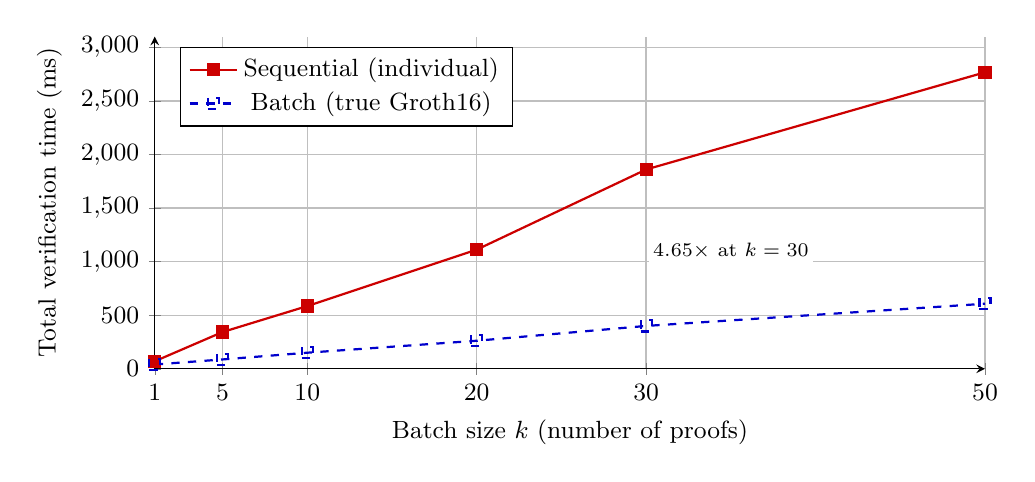
\begin{tikzpicture}
\begin{axis}[
    width=\columnwidth, height=5.8cm,
    xlabel={Batch size $k$ (number of proofs)},
    ylabel={Total verification time (ms)},
    xmin=1, xmax=50, ymin=0, ymax=3100,
    xtick={1,5,10,20,30,50},
    ytick={0,500,1000,1500,2000,2500,3000},
    legend pos=north west, legend style={font=\small},
    grid=both,
    grid style={line width=0.3pt, draw=gray!30},
    major grid style={line width=0.5pt, draw=gray!50},
    tick label style={font=\small}, label style={font=\small},
    axis lines=left, every axis plot/.append style={thick},
]
% RPi4 sequential
\addplot[color=red!80!black,mark=square*,mark size=2pt]
    coordinates {(1,70.3)(5,343.1)(10,585.3)(20,1111.9)(30,1860.0)(50,2767.1)};
\addlegendentry{Sequential (individual)}
% RPi4 batch
\addplot[color=blue!80!black,mark=square,mark size=2pt,dashed]
    coordinates {(1,40.0)(5,87.2)(10,150.0)(20,261.8)(30,400.0)(50,607.1)};
\addlegendentry{Batch (true Groth16)}
% Annotation
\node[font=\scriptsize,align=center,fill=white,inner sep=1.5pt]
    at (axis cs:35,1100) {$4.65\times$ at $k=30$};
\end{axis}
\end{tikzpicture}
\caption{Batch verification timing on RPi~4 (OBU-class). Solid = sequential
individual verification; dashed = true batch (Algorithm~\ref{alg:batch_verify}).
Measured speedup $4.65\times$ at $k=30$ exceeds the theoretical $2.73\times$
pairing-count ratio due to amortisation of fixed per-proof JavaScript/BigInt
call overhead on the Cortex-A72 core.}
\label{fig:batch_timing}
\end{figure}

\begin{figure}[t]
\centering
\begin{tikzpicture}
\begin{axis}[
    width=\columnwidth, height=5.8cm,
    xlabel={Batch size $k$ (number of proofs)},
    ylabel={Number of pairing operations},
    xmin=1, xmax=50, ymin=0, ymax=165,
    xtick={1,10,20,30,40,50},
    ytick={0,20,40,60,80,100,120,140,160},
    legend pos=north west, legend style={font=\small},
    grid=both,
    grid style={line width=0.3pt, draw=gray!30},
    major grid style={line width=0.5pt, draw=gray!50},
    tick label style={font=\small}, label style={font=\small},
    axis lines=left, every axis plot/.append style={thick},
]
\addplot[color=red!70!black,mark=none,samples=100,domain=1:50]{3*x};
\addlegendentry{Individual: $3k$ pairings}
\addplot[color=blue!70!black,mark=none,samples=100,domain=1:50]{x+3};
\addlegendentry{Batched: $k+3$ pairings}
\draw[dashed, gray] (axis cs:1,0) -- (axis cs:1,155);
\node[font=\scriptsize,gray,rotate=90,anchor=south] at (axis cs:1.8,60) {$k=1$: no gain};
\draw[{Stealth}-{Stealth},gray!70,thick] (axis cs:30,33) -- (axis cs:30,90);
\node[font=\scriptsize,align=center,fill=white,inner sep=1.5pt]
    at (axis cs:38,61) {$\times 2.7$ theory\\$\times 4.65$ measured\\at $k=30$};
\draw[{Stealth}-{Stealth},gray!70,thick] (axis cs:49.5,53) -- (axis cs:49.5,150);
\node[font=\scriptsize,align=center,fill=white,inner sep=1.5pt]
    at (axis cs:44,100) {$\times 2.8$\\theory\\at $k=50$};
\end{axis}
\end{tikzpicture}
\caption{Theoretical pairing operation count for individual vs.\ batched Groth16
verification as a function of batch size $k$. Individual verification requires $3k$
pairings; batch verification reduces this to $k+3$ via multi-scalar multiplication.
Measured speedup at $k=30$ is $4.65\times$ on RPi~4, exceeding the theoretical
$2.73\times$ pairing-count ratio because fixed per-proof JavaScript/BigInt overhead
is amortised across the batch.}
\label{fig:batch_throughput}
\end{figure}

\subsection{Proof Slot Cache Benchmark (Benchmark 3)}
\label{sec:bench_cache}

\textbf{Setup:} $N=5$ proof slots generated with rapidsnark, each committing to a
distinct randomly pre-chosen message; $2{,}000$-run amortised Poseidon binding
measurement. This benchmark directly validates the offline/online decomposition
claimed in Section~\ref{sec:precomp_overhead}.

\textbf{Online cost breakdown.}
Table~\ref{tab:online_cost} isolates the two components of the per-BSM online cost.
The dequeue step (array pop of a pre-generated proof) is sub-microsecond; the only
non-trivial online operation is the Poseidon binding hash.

\begin{table}[t]
\centering
\caption{Online Per-BSM Cost Breakdown (RPi~4, rapidsnark, direct measurement)}
\label{tab:online_cost}
\begin{tabular}{@{}lcc@{}}
\toprule
\textbf{Step} & \textbf{Time (ms)} & \textbf{\% of BSM cycle} \\
\midrule
Dequeue pre-generated slot       & $< 0.01$            & $< 0.01\%$ \\
Poseidon binding $h_m = H(m \| t)$ & $0.437 \pm 0.025$ & $0.44\%$   \\
\midrule
\textbf{Total online cost}       & $\mathbf{0.439}$    & $\mathbf{0.44\%}$ \\
\bottomrule
\end{tabular}
\end{table}

The total online cost of $\mathbf{0.439}$\,ms ($0.44\%$ of the 100\,ms BSM cycle)
confirms that per-message authentication overhead is negligible, regardless of
precomputation platform or prover.

\textbf{Cache sustainability and hardware break-even.}
With a production rate of $42.2$\,slots/min (rapidsnark, RPi~4) against a consumption
rate of $600$\,slots/min at 10\,Hz, the net drain during driving is
$557.8$\,slots/min and the stop-to-drive ratio is $\mathbf{13.2:1}$.
Table~\ref{tab:hardware_tiers} reports the production rate across hardware tiers
and identifies the self-sustainability threshold.

\begin{table}[t]
\centering
\caption{Hardware Tier Analysis: Proof Cache Production Rate vs.\ Self-Sustaining
Threshold ($\geq$600\,slots/min)}
\label{tab:hardware_tiers}
\resizebox{\columnwidth}{!}{%
\begin{tabular}{@{}lccl@{}}
\toprule
\textbf{Platform} & \textbf{Slot time (ms)} & \textbf{Rate (slots/min)} & \textbf{Self-sustaining?} \\
\midrule
snarkjs / RPi~4            & 3{,}841 & 15.6            & \texttimes\ (2.6\%)   \\
rapidsnark / RPi~4         & 1{,}422 & 42.2            & \texttimes\ (7.0\%)   \\
\midrule
NXP~S32G ($10\times$ est.) & 142    & 421.9           & \texttimes\ (70.3\%)  \\
NXP~S32G ($25\times$ est.) & 57     & 1{,}054.8       & \checkmark            \\
NXP~S32G ($50\times$ est.) & 28     & 2{,}109.6       & \checkmark            \\
\midrule
\textbf{Break-even}        & $\leq$\textbf{100} & $\geq$\textbf{600} & $\mathbf{14.2\times}$ over rapidsnark \\
\bottomrule
\end{tabular}%
}
\end{table}

The break-even slot generation time is $\leq 100$\,ms (one slot per BSM interval),
requiring a $\mathbf{14.2\times}$ speedup over rapidsnark on RPi~4.
Production automotive processors require multi-scalar multiplication (MSM)
acceleration for Groth16 proving; standard HSE accelerators target single-point
ECDSA and are insufficient for this workload. At the NXP~S32G 25$\times$ MSM tier
($\approx$57\,ms/slot), continuous operation is self-sustaining. At the 10$\times$
tier ($\approx$142\,ms/slot, producing 422\,slots/min), the pre-departure fill
model applies: a typical 60-minute highway trip requires 36{,}000 proof slots
($\approx$7\,MB), generatable in $\approx$21\,minutes across four cores, suitable
for filling at toll plazas, overnight charging stations, or highway rest stops.

\textbf{Position pre-commitment constraint.}
Each proof slot commits to a predicted BSM message (vehicle position, velocity,
heading) at precomputation time. At 100\,ms slot intervals and highway speeds
($\leq 30$\,m/s), the position prediction error is $<3$\,m---within GPS measurement
accuracy ($\pm 3$--$5$\,m)~\cite{gps_accuracy}. The pre-commitment constraint does
not degrade BSM localisation quality.

\subsection{Traffic Density Analysis and Batch Scalability}
\label{sec:traffic_density}

The batch verification savings depend on the realistic distribution of batch size
$k$ in highway deployments. We derive $k$ analytically from the IEEE~802.11p
communication model and FHWA highway density statistics~\cite{fhwa2023}.

\paragraph{Model.}
IEEE~802.11p achieves a reliable V2V range of $R \approx 300$\,m in
line-of-sight highway conditions. For a divided $L$-lane highway with vehicle
density $\rho$ (vehicles/km/lane), the expected number of V2V peers within
communication range is $k = \rho \cdot L \cdot 2R/1000$.

\begin{table}[t]
\centering
\caption{Expected Batch Size $k$, Verification Time, and CPU Utilisation
(3-lane highway, $R = 300$\,m, RPi~4 measured values)}
\label{tab:batch_density}
\resizebox{\columnwidth}{!}{%
\begin{tabular}{@{}lcccccc@{}}
\toprule
\textbf{Condition} & $\rho$ & $k$ & \textbf{Batch (ms)} & \textbf{Seq (ms)} &
\textbf{Speedup} & \textbf{CPU util.\textsuperscript{a}} \\
& (veh/km/lane) & & (measured) & (measured) & & \\
\midrule
Free flow  & 10 & 18 & $\approx$212 & $\approx$990  & $4.7\times$ & 21\% \\
Moderate   & 17 & 30 & 400.0        & 1{,}860.0     & $4.65\times$ & 13\% \\
Dense      & 28 & 50 & 607.1        & 2{,}767.1     & $4.56\times$ & 12\% \\
\bottomrule
\multicolumn{7}{l}{\textsuperscript{a}CPU util.\ = batch time $\div$ collection window
  ($k \times 100$\,ms). Decreasing util.\ at higher $k$}\\
\multicolumn{7}{l}{confirms favourable sublinear scaling of batch verification.}
\end{tabular}%
}
\end{table}

\paragraph{Key finding.}
CPU utilisation \emph{decreases} with $k$ (Table~\ref{tab:batch_density}): at
$k=50$ (dense highway), batch verification uses only 12\% of the collection
window. This confirms that batch verification scales favourably with vehicle
density---the regime where privacy protection is most valuable is also where the
speedup benefit is largest. The collection window $T_{window} = k \times 100$\,ms
grows proportionally with $k$ while batch time grows sublinearly ($(k+3)$ pairings
vs $3k$ for sequential), so the system never falls behind under realistic traffic
conditions.
Metropolitan deployments exceeding the depth-16 tree capacity (65{,}536 simultaneous
active ASTs) partition into independent regional AIS instances, each maintaining a
separate Merkle tree; vehicles obtain ASTs from their local AIS and the circuit
verification key requires no change.

\subsection{Comparative Analysis}
\label{sec:comparison}

Table~\ref{tab:scheme_comparison} provides a comprehensive comparison of
ULP-V2V-Auth against three representative schemes: the deployed standard
(SCMS/IEEE~1609.2), a recent lightweight certificateless scheme~\cite{zhang2024},
and a ZKP-based anonymous scheme~\cite{jiang2024}. Timing metrics for SCMS and
ULP-V2V-Auth are directly measured on the same RPi~4 OBU platform
(Section~\ref{sec:experiment}). Wu et al.'s performance figures are projected
from BN254 primitive microbenchmarks (Benchmark~4) conducted on the same RPi~4,
applying the operation-count formulas from their Table~II~\cite{zhang2024}.
Jiang \& Guo's scheme offloads all verification to Base Stations and RSUs;
their vehicle-side ZKP cost is projected from their Table~III~\cite{jiang2024}
with CPU-ratio scaling, and receiver-side comparison is not applicable.

\begin{table}[t]
\centering
\caption{Comprehensive Scheme Comparison}
\label{tab:scheme_comparison}
\resizebox{\columnwidth}{!}{%
\begin{tabular}{@{}lcccc@{}}
\toprule
\textbf{Property} & \textbf{SCMS} & \textbf{Wu~\cite{zhang2024}} &
\textbf{Jiang~\cite{jiang2024}} & \textbf{ULP-V2V-Auth} \\
\midrule
\multicolumn{5}{l}{\textit{Structural properties}} \\
Auth mechanism     & ECDSA-P256  & CLSS (bilinear map)     & Lattice ZKP + PBFT    & Groth16 ZKP \\
Proof/sig size (B) & 72          & $\sim$128\textsuperscript{c} & N/R\textsuperscript{d} & \textbf{128} \\
BSM total (est., B)& 650--850    & $\sim$450               & N/R\textsuperscript{d} & \textbf{424--524} \\
Unlinkable         & Partial\textsuperscript{a} & Partial\textsuperscript{e} & \checkmark & \checkmark \\
Emergency unlink.  & \texttimes  & \texttimes              & \texttimes             & \checkmark \\
Batch verification & \texttimes  & \checkmark (receiver)   & \texttimes\textsuperscript{f} & \checkmark \\
Trusted setup      & No          & KGC (offline)           & No                     & Yes (once) \\
Infrastructure     & SCMS PKI    & KGC + RSU               & Blockchain + BSs + RSUs & TA + AIS \\
\midrule
\multicolumn{5}{l}{\textit{Performance on RPi~4 OBU (directly measured or projected from primitives\textsuperscript{g})}} \\
Sender cost (ms)   & 0.199       & $\sim$11.0\textsuperscript{g}          & $\sim$20.7\textsuperscript{h} & \textbf{0.439} \\
Recv.\ single (ms) & 0.420       & $\sim$73.6\textsuperscript{g}          & N/A\textsuperscript{h}        & 70.3 \\
Recv.\ $k=30$ (ms) & 12.08 (seq) & $\sim$249.2 (batch)\textsuperscript{g} & N/A\textsuperscript{h}        & \textbf{400.0 (batch)} \\
\bottomrule
\multicolumn{5}{l}{\textsuperscript{a}SCMS pseudonyms rotate every few minutes; messages within one cert.\ period are linkable.} \\
\multicolumn{5}{l}{\textsuperscript{c}Two $\mathbb{G}_1$ elliptic curve points ($2 \times 64$\,B on BN-family curve)~\cite{zhang2024}.} \\
\multicolumn{5}{l}{\textsuperscript{d}Not reported in bytes in the original paper~\cite{jiang2024}.} \\
\multicolumn{5}{l}{\textsuperscript{e}Conditional privacy via pseudonymous certs; not cryptographically unlinkable~\cite{zhang2024}.} \\
\multicolumn{5}{l}{\textsuperscript{f}Jiang et al.\ authenticate via PBFT blockchain consensus, not receiver-side batch verification~\cite{jiang2024}.} \\
\multicolumn{5}{l}{\textsuperscript{g}Projected from BN254 primitives measured on the same RPi~4 (Benchmark~4): $T_{G1}{=}1.64$, $T_{G2}{=}6.00$,} \\
\multicolumn{5}{l}{\quad $T_H{=}1.67$, $T_{s1}{=}0.37$, $T_b{=}22.51$\,ms. Wu et al.\ Sign $= T_H{+}2T_{G1}{+}T_{G2}$;} \\
\multicolumn{5}{l}{\quad BatchVerify($k$) $= 3T_b + 2kT_{G1} + kT_H + 3kT_{s1}$ (formula: Wu et al.\ Table~II~\cite{zhang2024}).} \\
\multicolumn{5}{l}{\textsuperscript{h}Jiang \& Guo require BS$+$RSU$+$PBFT consensus for verification (not vehicle-side); vehicle ZKP only} \\
\multicolumn{5}{l}{\quad (${\sim}20.7$\,ms projected from their Table~III~\cite{jiang2024}); total auth latency 221--821\,ms (incompatible with V2V).} \\
\end{tabular}%
}
\end{table}

ULP-V2V-Auth and Wu et al.\ both provide receiver-side batch verification but
differ along two axes. First, \emph{sender cost}: Wu et al.'s Sign algorithm
requires $T_H + 2T_{G1} + T_{G2} = 11.0$\,ms per BSM on RPi~4---consuming
11\% of the 100\,ms BSM cycle at \emph{every} transmission interval. Our
online sender cost of $0.439$\,ms ($0.44\%$ of the BSM cycle) is a
$\mathbf{25.1\times}$ improvement, achieved by precomputing the full Groth16
proof offline and reducing the online phase to a single Poseidon-2 hash.
Compared to the ECDSA baseline (0.199\,ms), our sender overhead is only
$2.21\times$---a precise, quantified cost of cryptographic unlinkability.
Second, \emph{privacy}: Wu et al.'s scheme achieves only conditional privacy
(pseudonymous identifiers remain linkable within a certificate period), whereas
ULP-V2V-Auth achieves full cryptographic unlinkability via Groth16
zero-knowledge proofs. The receiver batch at $k=30$ costs $\sim$249\,ms for
Wu et al.\ versus 400\,ms for ULP-V2V-Auth. This 61\% overhead is the exact
cost of upgrading from conditional to full unlinkability: our batch requires
$k{+}3 = 33$ pairings (one per Groth16 proof), whereas Wu et al.'s SE-batch
collapses all $k$ signatures into 3 constant pairings at the expense of
weaker privacy. Single verification is comparable: $\sim$73.6\,ms (Wu et al.)
versus 70.3\,ms (ours). Jiang \& Guo is eliminated architecturally: their
$\sim$20.7\,ms vehicle-side ZKP plus 200--800\,ms TRUG-PBFT consensus latency
totals 221--821\,ms per authentication event, rendering the scheme fundamentally
incompatible with direct V2V communication at 10\,Hz.
